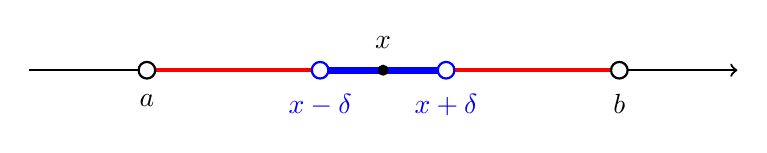
\begin{tikzpicture}[line width=0.8pt]
  \draw[->] (-0.5,0) -- (8.5,0);
  % the open interval (a,b)
  \draw[red, line width=1.6pt] (1,0) -- (7,0);
  \draw[fill=white] (1,0) circle (3pt) node[below=5pt] {$a$};
  \draw[fill=white] (7,0) circle (3pt) node[below=5pt] {$b$};
  % sub-interval centred at x
  \draw[blue, line width=2.4pt] (3.2,0) -- (4.8,0);
  \draw[blue, fill=white] (3.2,0) circle (3pt) node[below=5pt] {$x-\delta$};
  \draw[blue, fill=white] (4.8,0) circle (3pt) node[below=5pt] {$x+\delta$};
  \fill (4,0) circle (2pt) node[above=4pt] {$x$};
\end{tikzpicture}
